% Created by tikzDevice version 0.6.1 on 2011-06-03 22:21:19
% !TEX encoding = UTF-8 Unicode
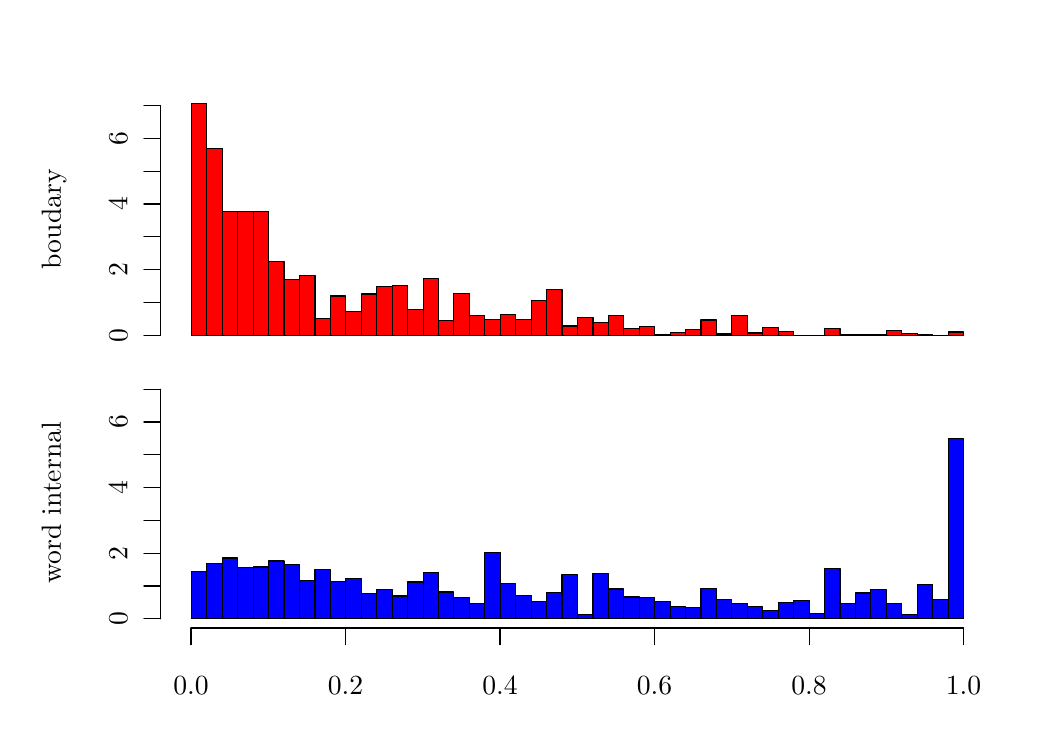
\begin{tikzpicture}[x=1pt,y=1pt]
\definecolor[named]{drawColor}{rgb}{0.00,0.00,0.00}
\definecolor[named]{fillColor}{rgb}{1.00,1.00,1.00}
\fill[color=fillColor,] (0,0) rectangle (361.35,252.94);
\begin{scope}
\path[clip] (  0.00,126.47) rectangle (361.35,252.94);
\definecolor[named]{drawColor}{rgb}{0.78,0.56,0.83}
\definecolor[named]{drawColor}{rgb}{0.00,0.00,0.00}

\node[rotate= 90.00,color=drawColor,anchor=base,inner sep=0pt, outer sep=0pt, scale=  1.00] at ( 12.00,183.71) {boudary%
};
\end{scope}
\begin{scope}
\path[clip] (  0.00,  0.00) rectangle (361.35,252.94);
\definecolor[named]{drawColor}{rgb}{0.78,0.56,0.83}
\definecolor[named]{drawColor}{rgb}{0.00,0.00,0.00}

\draw[color=drawColor,line cap=round,line join=round,fill opacity=0.00,] ( 48.00,141.82) -- ( 48.00,224.75);

\draw[color=drawColor,line cap=round,line join=round,fill opacity=0.00,] ( 48.00,141.82) -- ( 42.00,141.82);

\draw[color=drawColor,line cap=round,line join=round,fill opacity=0.00,] ( 48.00,153.67) -- ( 42.00,153.67);

\draw[color=drawColor,line cap=round,line join=round,fill opacity=0.00,] ( 48.00,165.52) -- ( 42.00,165.52);

\draw[color=drawColor,line cap=round,line join=round,fill opacity=0.00,] ( 48.00,177.36) -- ( 42.00,177.36);

\draw[color=drawColor,line cap=round,line join=round,fill opacity=0.00,] ( 48.00,189.21) -- ( 42.00,189.21);

\draw[color=drawColor,line cap=round,line join=round,fill opacity=0.00,] ( 48.00,201.05) -- ( 42.00,201.05);

\draw[color=drawColor,line cap=round,line join=round,fill opacity=0.00,] ( 48.00,212.90) -- ( 42.00,212.90);

\draw[color=drawColor,line cap=round,line join=round,fill opacity=0.00,] ( 48.00,224.75) -- ( 42.00,224.75);

\node[rotate= 90.00,color=drawColor,anchor=base,inner sep=0pt, outer sep=0pt, scale=  1.00] at ( 36.00,141.82) {0%
};

\node[rotate= 90.00,color=drawColor,anchor=base,inner sep=0pt, outer sep=0pt, scale=  1.00] at ( 36.00,165.52) {2%
};

\node[rotate= 90.00,color=drawColor,anchor=base,inner sep=0pt, outer sep=0pt, scale=  1.00] at ( 36.00,189.21) {4%
};

\node[rotate= 90.00,color=drawColor,anchor=base,inner sep=0pt, outer sep=0pt, scale=  1.00] at ( 36.00,212.90) {6%
};
\end{scope}
\begin{scope}
\path[clip] ( 48.00,138.47) rectangle (349.35,228.94);
\definecolor[named]{drawColor}{rgb}{0.78,0.56,0.83}
\definecolor[named]{drawColor}{rgb}{0.00,0.00,0.00}
\definecolor[named]{fillColor}{rgb}{1.00,0.00,0.00}

\draw[color=drawColor,line cap=round,line join=round,fill=fillColor,] ( 59.16,141.82) rectangle ( 64.74,225.59);

\draw[color=drawColor,line cap=round,line join=round,fill=fillColor,] ( 64.74,141.82) rectangle ( 70.32,209.41);

\draw[color=drawColor,line cap=round,line join=round,fill=fillColor,] ( 70.32,141.82) rectangle ( 75.90,186.38);

\draw[color=drawColor,line cap=round,line join=round,fill=fillColor,] ( 75.90,141.82) rectangle ( 81.48,186.45);

\draw[color=drawColor,line cap=round,line join=round,fill=fillColor,] ( 81.48,141.82) rectangle ( 87.06,186.54);

\draw[color=drawColor,line cap=round,line join=round,fill=fillColor,] ( 87.06,141.82) rectangle ( 92.64,168.39);

\draw[color=drawColor,line cap=round,line join=round,fill=fillColor,] ( 92.64,141.82) rectangle ( 98.22,161.98);

\draw[color=drawColor,line cap=round,line join=round,fill=fillColor,] ( 98.22,141.82) rectangle (103.81,163.49);

\draw[color=drawColor,line cap=round,line join=round,fill=fillColor,] (103.81,141.82) rectangle (109.39,147.89);

\draw[color=drawColor,line cap=round,line join=round,fill=fillColor,] (109.39,141.82) rectangle (114.97,155.98);

\draw[color=drawColor,line cap=round,line join=round,fill=fillColor,] (114.97,141.82) rectangle (120.55,150.36);

\draw[color=drawColor,line cap=round,line join=round,fill=fillColor,] (120.55,141.82) rectangle (126.13,156.71);

\draw[color=drawColor,line cap=round,line join=round,fill=fillColor,] (126.13,141.82) rectangle (131.71,159.25);

\draw[color=drawColor,line cap=round,line join=round,fill=fillColor,] (131.71,141.82) rectangle (137.29,159.76);

\draw[color=drawColor,line cap=round,line join=round,fill=fillColor,] (137.29,141.82) rectangle (142.87,151.16);

\draw[color=drawColor,line cap=round,line join=round,fill=fillColor,] (142.87,141.82) rectangle (148.45,162.21);

\draw[color=drawColor,line cap=round,line join=round,fill=fillColor,] (148.45,141.82) rectangle (154.03,147.00);

\draw[color=drawColor,line cap=round,line join=round,fill=fillColor,] (154.03,141.82) rectangle (159.61,156.84);

\draw[color=drawColor,line cap=round,line join=round,fill=fillColor,] (159.61,141.82) rectangle (165.19,148.94);

\draw[color=drawColor,line cap=round,line join=round,fill=fillColor,] (165.19,141.82) rectangle (170.77,147.61);

\draw[color=drawColor,line cap=round,line join=round,fill=fillColor,] (170.77,141.82) rectangle (176.35,149.19);

\draw[color=drawColor,line cap=round,line join=round,fill=fillColor,] (176.35,141.82) rectangle (181.93,147.47);

\draw[color=drawColor,line cap=round,line join=round,fill=fillColor,] (181.93,141.82) rectangle (187.51,154.24);

\draw[color=drawColor,line cap=round,line join=round,fill=fillColor,] (187.51,141.82) rectangle (193.09,158.27);

\draw[color=drawColor,line cap=round,line join=round,fill=fillColor,] (193.09,141.82) rectangle (198.67,145.14);

\draw[color=drawColor,line cap=round,line join=round,fill=fillColor,] (198.67,141.82) rectangle (204.26,148.05);

\draw[color=drawColor,line cap=round,line join=round,fill=fillColor,] (204.26,141.82) rectangle (209.84,146.47);

\draw[color=drawColor,line cap=round,line join=round,fill=fillColor,] (209.84,141.82) rectangle (215.42,149.08);

\draw[color=drawColor,line cap=round,line join=round,fill=fillColor,] (215.42,141.82) rectangle (221.00,144.27);

\draw[color=drawColor,line cap=round,line join=round,fill=fillColor,] (221.00,141.82) rectangle (226.58,145.09);

\draw[color=drawColor,line cap=round,line join=round,fill=fillColor,] (226.58,141.82) rectangle (232.16,142.21);

\draw[color=drawColor,line cap=round,line join=round,fill=fillColor,] (232.16,141.82) rectangle (237.74,142.91);

\draw[color=drawColor,line cap=round,line join=round,fill=fillColor,] (237.74,141.82) rectangle (243.32,143.76);

\draw[color=drawColor,line cap=round,line join=round,fill=fillColor,] (243.32,141.82) rectangle (248.90,147.29);

\draw[color=drawColor,line cap=round,line join=round,fill=fillColor,] (248.90,141.82) rectangle (254.48,142.25);

\draw[color=drawColor,line cap=round,line join=round,fill=fillColor,] (254.48,141.82) rectangle (260.06,148.97);

\draw[color=drawColor,line cap=round,line join=round,fill=fillColor,] (260.06,141.82) rectangle (265.64,142.60);

\draw[color=drawColor,line cap=round,line join=round,fill=fillColor,] (265.64,141.82) rectangle (271.22,144.73);

\draw[color=drawColor,line cap=round,line join=round,fill=fillColor,] (271.22,141.82) rectangle (276.80,143.23);

\draw[color=drawColor,line cap=round,line join=round,fill=fillColor,] (276.80,141.82) rectangle (282.38,141.86);

\draw[color=drawColor,line cap=round,line join=round,fill=fillColor,] (282.38,141.82) rectangle (287.96,141.82);

\draw[color=drawColor,line cap=round,line join=round,fill=fillColor,] (287.96,141.82) rectangle (293.54,144.34);

\draw[color=drawColor,line cap=round,line join=round,fill=fillColor,] (293.54,141.82) rectangle (299.12,141.93);

\draw[color=drawColor,line cap=round,line join=round,fill=fillColor,] (299.12,141.82) rectangle (304.71,141.88);

\draw[color=drawColor,line cap=round,line join=round,fill=fillColor,] (304.71,141.82) rectangle (310.29,141.98);

\draw[color=drawColor,line cap=round,line join=round,fill=fillColor,] (310.29,141.82) rectangle (315.87,143.53);

\draw[color=drawColor,line cap=round,line join=round,fill=fillColor,] (315.87,141.82) rectangle (321.45,142.36);

\draw[color=drawColor,line cap=round,line join=round,fill=fillColor,] (321.45,141.82) rectangle (327.03,142.16);

\draw[color=drawColor,line cap=round,line join=round,fill=fillColor,] (327.03,141.82) rectangle (332.61,141.82);

\draw[color=drawColor,line cap=round,line join=round,fill=fillColor,] (332.61,141.82) rectangle (338.19,142.96);
\end{scope}
\begin{scope}
\path[clip] ( 48.00, 36.00) rectangle (349.35,126.47);
\definecolor[named]{drawColor}{rgb}{0.78,0.56,0.83}
\end{scope}
\begin{scope}
\path[clip] (  0.00,  0.00) rectangle (361.35,126.47);
\definecolor[named]{drawColor}{rgb}{0.78,0.56,0.83}
\definecolor[named]{drawColor}{rgb}{0.00,0.00,0.00}

\node[rotate= 90.00,color=drawColor,anchor=base,inner sep=0pt, outer sep=0pt, scale=  1.00] at ( 12.00, 81.24) {word internal%
};
\end{scope}
\begin{scope}
\path[clip] (  0.00,  0.00) rectangle (361.35,252.94);
\definecolor[named]{drawColor}{rgb}{0.78,0.56,0.83}
\definecolor[named]{drawColor}{rgb}{0.00,0.00,0.00}

\draw[color=drawColor,line cap=round,line join=round,fill opacity=0.00,] ( 59.00, 36.00) -- (338.19, 36.00);

\draw[color=drawColor,line cap=round,line join=round,fill opacity=0.00,] ( 59.00, 36.00) -- ( 59.00, 30.00);

\draw[color=drawColor,line cap=round,line join=round,fill opacity=0.00,] (114.84, 36.00) -- (114.84, 30.00);

\draw[color=drawColor,line cap=round,line join=round,fill opacity=0.00,] (170.68, 36.00) -- (170.68, 30.00);

\draw[color=drawColor,line cap=round,line join=round,fill opacity=0.00,] (226.51, 36.00) -- (226.51, 30.00);

\draw[color=drawColor,line cap=round,line join=round,fill opacity=0.00,] (282.35, 36.00) -- (282.35, 30.00);

\draw[color=drawColor,line cap=round,line join=round,fill opacity=0.00,] (338.19, 36.00) -- (338.19, 30.00);

\node[color=drawColor,anchor=base,inner sep=0pt, outer sep=0pt, scale=  1.00] at ( 59.00, 12.00) {0.0%
};

\node[color=drawColor,anchor=base,inner sep=0pt, outer sep=0pt, scale=  1.00] at (114.84, 12.00) {0.2%
};

\node[color=drawColor,anchor=base,inner sep=0pt, outer sep=0pt, scale=  1.00] at (170.68, 12.00) {0.4%
};

\node[color=drawColor,anchor=base,inner sep=0pt, outer sep=0pt, scale=  1.00] at (226.51, 12.00) {0.6%
};

\node[color=drawColor,anchor=base,inner sep=0pt, outer sep=0pt, scale=  1.00] at (282.35, 12.00) {0.8%
};

\node[color=drawColor,anchor=base,inner sep=0pt, outer sep=0pt, scale=  1.00] at (338.19, 12.00) {1.0%
};

\draw[color=drawColor,line cap=round,line join=round,fill opacity=0.00,] ( 48.00, 39.35) -- ( 48.00,122.27);

\draw[color=drawColor,line cap=round,line join=round,fill opacity=0.00,] ( 48.00, 39.35) -- ( 42.00, 39.35);

\draw[color=drawColor,line cap=round,line join=round,fill opacity=0.00,] ( 48.00, 51.20) -- ( 42.00, 51.20);

\draw[color=drawColor,line cap=round,line join=round,fill opacity=0.00,] ( 48.00, 63.04) -- ( 42.00, 63.04);

\draw[color=drawColor,line cap=round,line join=round,fill opacity=0.00,] ( 48.00, 74.89) -- ( 42.00, 74.89);

\draw[color=drawColor,line cap=round,line join=round,fill opacity=0.00,] ( 48.00, 86.74) -- ( 42.00, 86.74);

\draw[color=drawColor,line cap=round,line join=round,fill opacity=0.00,] ( 48.00, 98.58) -- ( 42.00, 98.58);

\draw[color=drawColor,line cap=round,line join=round,fill opacity=0.00,] ( 48.00,110.43) -- ( 42.00,110.43);

\draw[color=drawColor,line cap=round,line join=round,fill opacity=0.00,] ( 48.00,122.27) -- ( 42.00,122.27);

\node[rotate= 90.00,color=drawColor,anchor=base,inner sep=0pt, outer sep=0pt, scale=  1.00] at ( 36.00, 39.35) {0%
};

\node[rotate= 90.00,color=drawColor,anchor=base,inner sep=0pt, outer sep=0pt, scale=  1.00] at ( 36.00, 63.04) {2%
};

\node[rotate= 90.00,color=drawColor,anchor=base,inner sep=0pt, outer sep=0pt, scale=  1.00] at ( 36.00, 86.74) {4%
};

\node[rotate= 90.00,color=drawColor,anchor=base,inner sep=0pt, outer sep=0pt, scale=  1.00] at ( 36.00,110.43) {6%
};
\end{scope}
\begin{scope}
\path[clip] ( 48.00, 36.00) rectangle (349.35,126.47);
\definecolor[named]{drawColor}{rgb}{0.78,0.56,0.83}
\definecolor[named]{drawColor}{rgb}{0.00,0.00,0.00}
\definecolor[named]{fillColor}{rgb}{0.00,0.00,1.00}

\draw[color=drawColor,line cap=round,line join=round,fill=fillColor,] ( 59.16, 39.35) rectangle ( 64.74, 56.41);

\draw[color=drawColor,line cap=round,line join=round,fill=fillColor,] ( 64.74, 39.35) rectangle ( 70.32, 59.33);

\draw[color=drawColor,line cap=round,line join=round,fill=fillColor,] ( 70.32, 39.35) rectangle ( 75.90, 61.30);

\draw[color=drawColor,line cap=round,line join=round,fill=fillColor,] ( 75.90, 39.35) rectangle ( 81.48, 57.92);

\draw[color=drawColor,line cap=round,line join=round,fill=fillColor,] ( 81.48, 39.35) rectangle ( 87.06, 58.05);

\draw[color=drawColor,line cap=round,line join=round,fill=fillColor,] ( 87.06, 39.35) rectangle ( 92.64, 60.24);

\draw[color=drawColor,line cap=round,line join=round,fill=fillColor,] ( 92.64, 39.35) rectangle ( 98.22, 58.86);

\draw[color=drawColor,line cap=round,line join=round,fill=fillColor,] ( 98.22, 39.35) rectangle (103.81, 53.13);

\draw[color=drawColor,line cap=round,line join=round,fill=fillColor,] (103.81, 39.35) rectangle (109.39, 57.05);

\draw[color=drawColor,line cap=round,line join=round,fill=fillColor,] (109.39, 39.35) rectangle (114.97, 52.75);

\draw[color=drawColor,line cap=round,line join=round,fill=fillColor,] (114.97, 39.35) rectangle (120.55, 53.97);

\draw[color=drawColor,line cap=round,line join=round,fill=fillColor,] (120.55, 39.35) rectangle (126.13, 48.40);

\draw[color=drawColor,line cap=round,line join=round,fill=fillColor,] (126.13, 39.35) rectangle (131.71, 50.00);

\draw[color=drawColor,line cap=round,line join=round,fill=fillColor,] (131.71, 39.35) rectangle (137.29, 47.58);

\draw[color=drawColor,line cap=round,line join=round,fill=fillColor,] (137.29, 39.35) rectangle (142.87, 52.65);

\draw[color=drawColor,line cap=round,line join=round,fill=fillColor,] (142.87, 39.35) rectangle (148.45, 56.14);

\draw[color=drawColor,line cap=round,line join=round,fill=fillColor,] (148.45, 39.35) rectangle (154.03, 49.01);

\draw[color=drawColor,line cap=round,line join=round,fill=fillColor,] (154.03, 39.35) rectangle (159.61, 46.97);

\draw[color=drawColor,line cap=round,line join=round,fill=fillColor,] (159.61, 39.35) rectangle (165.19, 44.71);

\draw[color=drawColor,line cap=round,line join=round,fill=fillColor,] (165.19, 39.35) rectangle (170.77, 63.45);

\draw[color=drawColor,line cap=round,line join=round,fill=fillColor,] (170.77, 39.35) rectangle (176.35, 51.96);

\draw[color=drawColor,line cap=round,line join=round,fill=fillColor,] (176.35, 39.35) rectangle (181.93, 47.86);

\draw[color=drawColor,line cap=round,line join=round,fill=fillColor,] (181.93, 39.35) rectangle (187.51, 45.68);

\draw[color=drawColor,line cap=round,line join=round,fill=fillColor,] (187.51, 39.35) rectangle (193.09, 48.87);

\draw[color=drawColor,line cap=round,line join=round,fill=fillColor,] (193.09, 39.35) rectangle (198.67, 55.24);

\draw[color=drawColor,line cap=round,line join=round,fill=fillColor,] (198.67, 39.35) rectangle (204.26, 40.94);

\draw[color=drawColor,line cap=round,line join=round,fill=fillColor,] (204.26, 39.35) rectangle (209.84, 55.72);

\draw[color=drawColor,line cap=round,line join=round,fill=fillColor,] (209.84, 39.35) rectangle (215.42, 50.10);

\draw[color=drawColor,line cap=round,line join=round,fill=fillColor,] (215.42, 39.35) rectangle (221.00, 47.23);

\draw[color=drawColor,line cap=round,line join=round,fill=fillColor,] (221.00, 39.35) rectangle (226.58, 47.11);

\draw[color=drawColor,line cap=round,line join=round,fill=fillColor,] (226.58, 39.35) rectangle (232.16, 45.46);

\draw[color=drawColor,line cap=round,line join=round,fill=fillColor,] (232.16, 39.35) rectangle (237.74, 43.71);

\draw[color=drawColor,line cap=round,line join=round,fill=fillColor,] (237.74, 39.35) rectangle (243.32, 43.54);

\draw[color=drawColor,line cap=round,line join=round,fill=fillColor,] (243.32, 39.35) rectangle (248.90, 50.16);

\draw[color=drawColor,line cap=round,line join=round,fill=fillColor,] (248.90, 39.35) rectangle (254.48, 46.23);

\draw[color=drawColor,line cap=round,line join=round,fill=fillColor,] (254.48, 39.35) rectangle (260.06, 44.98);

\draw[color=drawColor,line cap=round,line join=round,fill=fillColor,] (260.06, 39.35) rectangle (265.64, 43.75);

\draw[color=drawColor,line cap=round,line join=round,fill=fillColor,] (265.64, 39.35) rectangle (271.22, 42.47);

\draw[color=drawColor,line cap=round,line join=round,fill=fillColor,] (271.22, 39.35) rectangle (276.80, 45.10);

\draw[color=drawColor,line cap=round,line join=round,fill=fillColor,] (276.80, 39.35) rectangle (282.38, 45.87);

\draw[color=drawColor,line cap=round,line join=round,fill=fillColor,] (282.38, 39.35) rectangle (287.96, 41.27);

\draw[color=drawColor,line cap=round,line join=round,fill=fillColor,] (287.96, 39.35) rectangle (293.54, 57.52);

\draw[color=drawColor,line cap=round,line join=round,fill=fillColor,] (293.54, 39.35) rectangle (299.12, 44.74);

\draw[color=drawColor,line cap=round,line join=round,fill=fillColor,] (299.12, 39.35) rectangle (304.71, 48.67);

\draw[color=drawColor,line cap=round,line join=round,fill=fillColor,] (304.71, 39.35) rectangle (310.29, 49.80);

\draw[color=drawColor,line cap=round,line join=round,fill=fillColor,] (310.29, 39.35) rectangle (315.87, 44.98);

\draw[color=drawColor,line cap=round,line join=round,fill=fillColor,] (315.87, 39.35) rectangle (321.45, 41.02);

\draw[color=drawColor,line cap=round,line join=round,fill=fillColor,] (321.45, 39.35) rectangle (327.03, 51.62);

\draw[color=drawColor,line cap=round,line join=round,fill=fillColor,] (327.03, 39.35) rectangle (332.61, 46.39);

\draw[color=drawColor,line cap=round,line join=round,fill=fillColor,] (332.61, 39.35) rectangle (338.19,104.35);
\end{scope}
\end{tikzpicture}
